% Extension decision tree — 5-question stop-at-first-match ladder.
% Pedagogy pass (Mayer/Tufte/Miller): terse labels (<=7 words, no parentheticals);
% no file-path / caveat subtitles (those live in the prose); color reserved for the
% CATEGORY endpoints (command=blue, skill=green, hook=rose, MCP=plum, plugin=gold);
% decision diamonds are NEUTRAL so the scaffolding recedes. Warm-Tol brand hues.
\documentclass[tikz,border=4mm]{standalone}
\usepackage{tikz}
\usetikzlibrary{positioning, shapes.geometric, arrows.meta, calc}

\definecolor{warmblue}{HTML}{3B6FA0}
\definecolor{warmrose}{HTML}{C06858}
\definecolor{warmgreen}{HTML}{4A7E3F}
\definecolor{warmplum}{HTML}{8A4E82}
\definecolor{warmgold}{HTML}{C09840}

\begin{document}
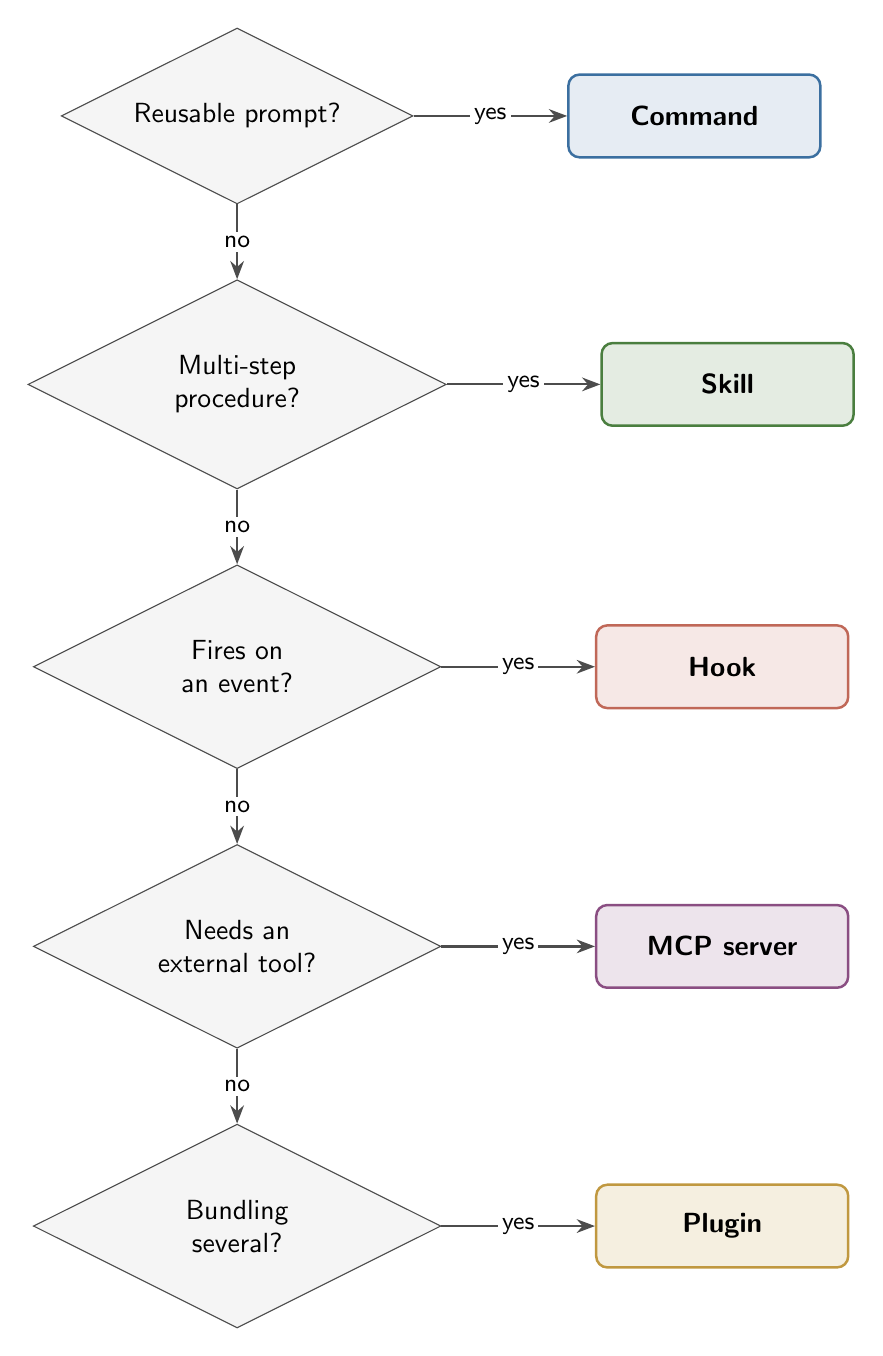
\begin{tikzpicture}[
  font=\sffamily,
  node distance=0.95cm and 1.95cm,
  question/.style={
    draw=gray!60!black, fill=gray!8, diamond, aspect=2.0,
    inner sep=4pt, align=center, text width=3.0cm, font=\sffamily
  },
  ep/.style={
    rounded corners=4pt, minimum width=3.2cm, minimum height=1.05cm,
    inner sep=6pt, align=center, font=\sffamily\bfseries, line width=0.9pt
  },
  epblue/.style={ep, draw=warmblue, fill=warmblue!13},
  epgreen/.style={ep, draw=warmgreen, fill=warmgreen!15},
  eprose/.style={ep, draw=warmrose, fill=warmrose!15},
  epplum/.style={ep, draw=warmplum, fill=warmplum!15},
  epgold/.style={ep, draw=warmgold, fill=warmgold!16},
  arrow/.style={-Stealth, thick, draw=gray!60!black},
  arrowlabel/.style={font=\sffamily\small, fill=white, inner sep=1.5pt},
]

\node[question] (q1) {Reusable prompt?};
\node[epblue, right=of q1] (cmd) {Command};

\node[question, below=of q1] (q2) {Multi-step \\ procedure?};
\node[epgreen, right=of q2] (skill) {Skill};

\node[question, below=of q2] (q3) {Fires on \\ an event?};
\node[eprose, right=of q3] (hook) {Hook};

\node[question, below=of q3] (q4) {Needs an \\ external tool?};
\node[epplum, right=of q4] (mcp) {MCP server};

\node[question, below=of q4] (q5) {Bundling \\ several?};
\node[epgold, right=of q5] (plug) {Plugin};

\draw[arrow] (q1) -- node[arrowlabel] {yes} (cmd);
\draw[arrow] (q1) -- node[arrowlabel] {no} (q2);
\draw[arrow] (q2) -- node[arrowlabel] {yes} (skill);
\draw[arrow] (q2) -- node[arrowlabel] {no} (q3);
\draw[arrow] (q3) -- node[arrowlabel] {yes} (hook);
\draw[arrow] (q3) -- node[arrowlabel] {no} (q4);
\draw[arrow] (q4) -- node[arrowlabel] {yes} (mcp);
\draw[arrow] (q4) -- node[arrowlabel] {no} (q5);
\draw[arrow] (q5) -- node[arrowlabel] {yes} (plug);

\end{tikzpicture}
\end{document}
